% -*- Mode:TeX -*-

%% IMPORTANT: The official thesis specifications are available at:
%%            http://libraries.mit.edu/archives/thesis-specs/
%%
%%            Please verify your thesis' formatting and copyright
%%            assignment before submission.  If you notice any
%%            discrepancies between these templates and the 
%%            MIT Libraries' specs, please let us know
%%            by e-mailing thesis@mit.edu

%% The documentclass options along with the pagestyle can be used to generate
%% a technical report, a draft copy, or a regular thesis.  You may need to
%% re-specify the pagestyle after you \include  cover.tex.  For more
%% information, see the first few lines of mitthesis.cls. 

%\documentclass[12pt,vi,twoside]{mitthesis}
%%
%%  If you want your thesis copyright to you instead of MIT, use the
%%  ``vi'' option, as above.
%%
%\documentclass[12pt,twoside,leftblank]{mitthesis}
%%
%% If you want blank pages before new chapters to be labelled ``This
%% Page Intentionally Left Blank'', use the ``leftblank'' option, as
%% above. 

\documentclass[12pt,oneside]{mitthesis}
\usepackage{lgrind}
\usepackage{graphicx}
\usepackage{algpseudocode}
\usepackage{algorithmicx}
\usepackage{algorithm}
\usepackage{float}
\usepackage{qtree}
\usepackage{listings}
\usepackage{color}
\usepackage{newfloat}
\usepackage{hyperref}
\usepackage{amsthm}
\usepackage{textcomp}
\usepackage{cleveref}[2012/02/15]
\crefformat{footnote}{#2\footnotemark[#1]#3}

\usepackage{url}
\newfloat{algorithm}{t}{lop}
\floatname{algorithm}{Algorithm}
\usepackage{subfig}

\lstset{captionpos=b,
        frame=tb,
        basicstyle=\scriptsize\ttfamily,
        showstringspaces=false,
        keepspaces=true}
\lstdefinestyle{matlab} {
        language=Matlab,
        keywordstyle=\color{blue},
        commentstyle=\color[rgb]{0.13,0.55,0.13}\em,
        stringstyle=\color[rgb]{0.7,0,0} }

\DeclareFloatingEnvironment[fileext=lod]{diagram}

% "define" Scala
\lstdefinelanguage{scala}{
  morekeywords={abstract,case,catch,class,def,%
    do,else,extends,false,final,finally,%
    for,if,implicit,import,match,mixin,%
    new,null,object,override,package,%
    private,protected,requires,return,sealed,%
    super,this,throw,trait,true,try,%
    type,val,var,while,with,yield},
  otherkeywords={=>,<-,<\%,<:,>:,\#,@},
  sensitive=true,
  morecomment=[l]{//},
  morecomment=[n]{/*}{*/},
  morestring=[b]",
  morestring=[b]',
  morestring=[b]"""
}


\newtheorem{theorem}{Theorem}[section]
\newtheorem{lemma}[theorem]{Lemma}
\newtheorem{proposition}[theorem]{Proposition}
\newtheorem{corollary}[theorem]{Corollary}
\newtheorem{definition}[theorem]{Definition}

\def\definitionautorefname{Definition}

\renewcommand{\algorithmicrequire}{\textbf{Input:}}
\renewcommand{\algorithmicensure}{\textbf{Output:}}



%----------------------------------------------------------------------------------
%----------------------------------------------------------------------------------
\definecolor{lightgray}{rgb}{.8,.8,.8}  % define new color
% \sethlcolor{lightgray}  % define highlight and mynote color

%--- defining default vspaces ---
\newcommand{\vspacebfigure}{\vspace{0mm}}   % vspace before caption of figure
\newcommand{\vspaceafigure}{\vspace{-4mm}}   % vspace after caption of figure

%--- define my paragraph ---
\newcommand{\myparagraph}[1]{\vspace{2mm}\noindent\textbf{#1}}

\newcommand{\myparagraphnobold}[1]{\vspace{2mm}\noindent #1}

%\newcommand{\para}[1]{\paragraph*{#1}}
\newcommand{\para}[1]{\vspace{2mm}\noindent\textbf{#1}}

%--- general gray box for notes ---
\newcommand{\mynote}[1]{\par\noindent\colorbox{lightgray}{\parbox{\linewidth}{#1}}}
\newcommand{\mybignote}[1]{\mynote{\centering --- \textbf{#1} ---}\\[-1mm]}
% \renewcommand{\mynote}[1]{}

%--- comments from authors ---
\newcommand{\mynotesf}[1]{\mynote{\textsf{#1}}}
%--- comments from authors ---
\newcommand{\reminder}[1]{[[[\vadjust{\vbox to0pt{\vss\hbox to0pt{\hss{\Large $\Longrightarrow$}}}}{{\textsf{\small #1}}}]]]}
% \renewcommand{\reminder}[1]{}
% \newcommand{\reminder}[1]{}
\newcommand{\AK}[1]{\textcolor{red}{\mynotesf{AK:~#1}}}
\newcommand{\TODO}[1]{\textcolor{red}{\mynotesf{TODO:~#1}}}
%% placeholder for a variable or constant
\newcommand{\ph}[1]{\texttt{#1}}


\lstset{
    breaklines = true
}

% New definitions
\algnewcommand\algorithmicswitch{\textbf{match}}
\algnewcommand\algorithmiccase{\textbf{case}}
\algnewcommand\algorithmicassert{\texttt{assert}}
\algnewcommand\Or{\textbf{or}}
\algnewcommand\And{\textbf{and}}
\algnewcommand\Assert[1]{\State \algorithmicassert(#1)}%
% New "environments"
\algdef{SE}[SWITCH]{Switch}{EndSwitch}[1]{\algorithmicswitch\ #1\ \algorithmicdo}{\algorithmicend\ \algorithmicswitch}%
\algdef{SE}[CASE]{Case}{EndCase}[1]{\algorithmiccase\ #1}{\algorithmicend\ \algorithmiccase}%
\algtext*{EndSwitch}%
\algtext*{EndCase}%

\renewcommand\algorithmicthen{}
\renewcommand\algorithmicdo{}
\algtext*{EndWhile}% Remove "end while" text
\algtext*{EndIf}% Remove "end if" text
\algtext*{EndFor}% Remove "end for" text

\algnewcommand{\Inputs}[1]{%
  \State \textbf{Inputs:}
  \Statex \hspace*{\algorithmicindent}\parbox[t]{.8\linewidth}{\raggedright #1}
}

\algnewcommand{\Initialize}[1]{%
  \State \textbf{Initialize:}
  \Statex \hspace*{\algorithmicindent}\parbox[t]{.8\linewidth}{\raggedright #1}
}

\pagestyle{plain}

%% This bit allows you to either specify only the files which you wish to
%% process, or `all' to process all files which you \include.
%% Krishna Sethuraman (1990).

\begin{document}

% Some departments (e.g. 5) require an additional signature page.  See
% signature.tex for more information and uncomment the following line if
% applicable.
% % -*- Mode:TeX -*-
%
% Some departments (e.g. Chemistry) require an additional cover page
% with signatures of the thesis committee.  Please check with your
% thesis advisor or other appropriate person to determine if such a 
% page is required for your thesis.  
%
% If you choose not to use the "titlepage" environment, a \newpage
% commands, and several \vspace{\fill} commands may be necessary to
% achieve the required spacing.  The \signature command is defined in
% the "mitthesis" class
%
% The following sample appears courtesy of Ben Kaduk <kaduk@mit.edu> and
% was used in his June 2012 doctoral thesis in Chemistry. 

\begin{titlepage}
\begin{large}
This doctoral thesis has been examined by a Committee of the Department
of Chemistry as follows:

\signature{Professor Jianshu Cao}{Chairman, Thesis Committee \\
   Professor of Chemistry}

\signature{Professor Troy Van Voorhis}{Thesis Supervisor \\
   Associate Professor of Chemistry}

\signature{Professor Robert W. Field}{Member, Thesis Committee \\
   Haslam and Dewey Professor of Chemistry}
\end{large}
\end{titlepage}


\pagestyle{plain}
% -*-latex-*-
% 
% For questions, comments, concerns or complaints:
% thesis@mit.edu
% 
%
% $Log: cover.tex,v $
% Revision 1.8  2008/05/13 15:02:15  jdreed
% Degree month is June, not May.  Added note about prevdegrees.
% Arthur Smith's title updated
%
% Revision 1.7  2001/02/08 18:53:16  boojum
% changed some \newpages to \cleardoublepages
%
% Revision 1.6  1999/10/21 14:49:31  boojum
% changed comment referring to documentstyle
%
% Revision 1.5  1999/10/21 14:39:04  boojum
% *** empty log message ***
%
% Revision 1.4  1997/04/18  17:54:10  othomas
% added page numbers on abstract and cover, and made 1 abstract
% page the default rather than 2.  (anne hunter tells me this
% is the new institute standard.)
%
% Revision 1.4  1997/04/18  17:54:10  othomas
% added page numbers on abstract and cover, and made 1 abstract
% page the default rather than 2.  (anne hunter tells me this
% is the new institute standard.)
%
% Revision 1.3  93/05/17  17:06:29  starflt
% Added acknowledgements section (suggested by tompalka)
% 
% Revision 1.2  92/04/22  13:13:13  epeisach
% Fixes for 1991 course 6 requirements
% Phrase "and to grant others the right to do so" has been added to 
% permission clause
% Second copy of abstract is not counted as separate pages so numbering works
% out
% 
% Revision 1.1  92/04/22  13:08:20  epeisach

% NOTE:
% These templates make an effort to conform to the MIT Thesis specifications,
% however the specifications can change.  We recommend that you verify the
% layout of your title page with your thesis advisor and/or the MIT 
% Libraries before printing your final copy.
\title{Workflow Management System for Stratosphere}

\author{Suryamita Harindrari}
% If you wish to list your previous degrees on the cover page, use the 
% previous degrees command:
%       \prevdegrees{A.A., Harvard University (1985)}
% You can use the \\ command to list multiple previous degrees
%       \prevdegrees{B.S., University of California (1978) \\
%                    S.M., Massachusetts Institute of Technology (1981)}
\department{Department of Computer Science and Electrical Engineering}

% If the thesis is for two degrees simultaneously, list them both
% separated by \and like this:
% \degree{Doctor of Philosophy \and Master of Science}
\degree{Master of Science in Computer Science and Engineering}

% As of the 2007-08 academic year, valid degree months are September, 
% February, or June.  The default is June.
\degreemonth{July}
\degreeyear{2014}
\thesisdate{July 31, 2014}

%% By default, the thesis will be copyrighted to MIT.  If you need to copyright
%% the thesis to yourself, just specify the `vi' documentclass option.  If for
%% some reason you want to exactly specify the copyright notice text, you can
%% use the \copyrightnoticetext command.  
%\copyrightnoticetext{\copyright IBM, 1990.  Do not open till Xmas.}

% If there is more than one supervisor, use the \supervisor command
% once for each.
\supervisor{Asterios Katsifodimos}{Associate Professor}

% This is the department committee chairman, not the thesis committee
% chairman.  You should replace this with your Department's Committee
% Chairman.
\chairman{Ralf Detlef-Kutsche}{Chairman, Department Committee on Graduate Theses}

% Make the titlepage based on the above information.  If you need
% something special and can't use the standard form, you can specify
% the exact text of the titlepage yourself.  Put it in a titlepage
% environment and leave blank lines where you want vertical space.
% The spaces will be adjusted to fill the entire page.  The dotted
% lines for the signatures are made with the \signature command.
\maketitle

% The abstractpage environment sets up everything on the page except
% the text itself.  The title and other header material are put at the
% top of the page, and the supervisors are listed at the bottom.  A
% new page is begun both before and after.  Of course, an abstract may
% be more than one page itself.  If you need more control over the
% format of the page, you can use the abstract environment, which puts
% the word "Abstract" at the beginning and single spaces its text.

%% You can either \input (*not* \include) your abstract file, or you can put
%% the text of the abstract directly between the \begin{abstractpage} and
%% \end{abstractpage} commands.

% First copy: start a new page, and save the page number.
\cleardoublepage
% Uncomment the next line if you do NOT want a page number on your
% abstract and acknowledgments pages.
% \pagestyle{empty}
\setcounter{savepage}{\thepage}
\begin{abstractpage}
% $Log: abstract.tex,v $
% Revision 1.1  93/05/14  14:56:25  starflt
% Initial revision
% 
% Revision 1.1  90/05/04  10:41:01  lwvanels
% Initial revision
% 
%
%% The text of your abstract and nothing else (other than comments) goes here.
%% It will be single-spaced and the rest of the text that is supposed to go on
%% the abstract page will be generated by the abstractpage environment.  This
%% file should be \input (not \include 'd) from cover.tex.
In this thesis, we design and develop the preliminary scope of a Workflow Management System (WMS) which is aimed to work on top of Stratosphere, one of the emerging large-scale data processing frameworks. The WMS is developed by means of a Domain Specific Language (DSL) which is deeply embedded in Scala high-level programming language. The aim of this workflow DSL is to enable the progammer to define the workflow of complex use cases without having to manually specify the dependencies between the tasks in the workflow. Control Flow and data dependencies are automatically detected by static analysis on the program code using our compiler framework. 

The goal to translate the user program written in our DSL to the target code is achieved through the following three stages: (1) generate a control flow graph as an intermediate representation (IR) from Abstract Syntax Trees (AST) of the program, (2) perform data flow analysis to enrich the graph with data dependencies information, and (3) generate code or job scripts for the underlying system. This research develops the algorithm for each of three stages as well as the implementation of the first stage of the overall process. In the evaluation, we argue over the advantages of this DSL compared to related WMS work in terms of productivity and generality i.e. extensibility to other underlying platforms.

\end{abstractpage}

% Additional copy: start a new page, and reset the page number.  This way,
% the second copy of the abstract is not counted as separate pages.
% Uncomment the next 6 lines if you need two copies of the abstract
% page.
% \setcounter{page}{\thesavepage}
% \begin{abstractpage}
% % $Log: abstract.tex,v $
% Revision 1.1  93/05/14  14:56:25  starflt
% Initial revision
% 
% Revision 1.1  90/05/04  10:41:01  lwvanels
% Initial revision
% 
%
%% The text of your abstract and nothing else (other than comments) goes here.
%% It will be single-spaced and the rest of the text that is supposed to go on
%% the abstract page will be generated by the abstractpage environment.  This
%% file should be \input (not \include 'd) from cover.tex.
In this thesis, we design and develop the preliminary scope of a Workflow Management System (WMS) which is aimed to work on top of Stratosphere, one of the emerging large-scale data processing frameworks. The WMS is developed by means of a Domain Specific Language (DSL) which is deeply embedded in Scala high-level programming language. The aim of this workflow DSL is to enable the progammer to define the workflow of complex use cases without having to manually specify the dependencies between the tasks in the workflow. Control Flow and data dependencies are automatically detected by static analysis on the program code using our compiler framework. 

The goal to translate the user program written in our DSL to the target code is achieved through the following three stages: (1) generate a control flow graph as an intermediate representation (IR) from Abstract Syntax Trees (AST) of the program, (2) perform data flow analysis to enrich the graph with data dependencies information, and (3) generate code or job scripts for the underlying system. This research develops the algorithm for each of three stages as well as the implementation of the first stage of the overall process. In the evaluation, we argue over the advantages of this DSL compared to related WMS work in terms of productivity and generality i.e. extensibility to other underlying platforms.

% \end{abstractpage}

\cleardoublepage

\section*{Acknowledgments}

This is the acknowledgements section.  You should replace this with your
own acknowledgements.

%%%%%%%%%%%%%%%%%%%%%%%%%%%%%%%%%%%%%%%%%%%%%%%%%%%%%%%%%%%%%%%%%%%%%%
% -*-latex-*-

  % -*- Mode:TeX -*-
%% This file simply contains the commands that actually generate the table of
%% contents and lists of figures and tables.  You can omit any or all of
%% these files by simply taking out the appropriate command.  For more
%% information on these files, see appendix C.3.3 of the LaTeX manual. 
\tableofcontents
\newpage
\listoffigures
\newpage
\listoftables


%% This is an example first chapter.  You should put chapter/appendix that you
%% write into a separate file, and add a line \include{yourfilename} to
%% main.tex, where `yourfilename.tex' is the name of the chapter/appendix file.
%% You can process specific files by typing their names in at the 
%% \files=
%% prompt when you run the file main.tex through LaTeX.
\chapter{Introduction}
With the advancement of Big Data Analytics, data engineers are building more and more complex applications to manage and process large data sets on distributed resources. Such complex application scenarios require means in order to compose and execute complex workflows. Workflows automate procedures that users would otherwise need to carry out manually \cite{deelman2009workflows}. A workflow refers to a sequence of steps or computations that a user would like to perform 
\footnote{\label{crobak}http://www.crobak.org/2012/07/workflow-engines-for-hadoop}. As an example, within a Hadoop \footnote{\label{hadoop}http://hadoop.apache.org/.} cluster, a user may need to export the production databases and load the data to the Hadoop File System (HDFS) as the first step. The second step would be to run a MapReduce job to clean up the data and step three would be a set of operations that run in parallel to count and filter the data. A workflow is intended to map all of the different operations together. Such a workflow is usually represented as a Directed Acyclic Graph (DAG) where the nodes can be tasks or control flow structures and edges represent the relationships between tasks, namely task or data dependency. A Workflow Management System (WMS) is a system that allows users and developers to create, define, run, and delete a workflow \cref{crobak}. 
	
As an introduction to what a workflow may look like, we will walk through two different use cases that are representative use cases in the Big Data environment. The first use case is Analytics/Data Warehousing. A workflow in this first use case consists of the following steps: (1) load the logs into the Fact tables, (2) load the database backups into the Dimension tables, (3) compute the aggregations and perform rollups/cubes inside Hadoop for instance, (4) load the data into a low latency store, and (4) in the end, perform the analytics using a Dashboard and BI tools. The second use case is related to machine learning or collaborative filtering. A workflow in this use case consists of the followings steps: (1) load the logs and database backups into the HDFS, (2) perform the collaborative filtering and machine learning computation, (3) produce the production datasets in Hadoop, for example, (4) perform the sanity check of the production data set, and (5) at the end, load the cleaned data to production data store \cref{crobak}.

\section{Overview}
The current existing WMS, which will be explored further in the related work section, mainly act as a “glue” of simple jobs defined by the developer. Data dependencies and control flow in the workflow (e.g. decision making, looping, and branching) are specified manually in the model. This manual job causes a large overhead and confusion to the developer. It would be convenient if the WMS is able to automatically detect the control flow and data dependencies between the tasks based on pure program code. 

The overall goal of this thesis is to design and develop a prototype of WMS that works on top of Stratosphere, the Big Data Analytics platform developed by DIMA in TU Berlin. The approach that will be taken to define the workflow specification is to develop a Domain Specific Language (DSL) on top of Scala \cite{odersky2004overview}, a high-level functional programming language. The idea is to build a WMS that will take a Scala program which defines a set of tasks associated with each other in a given sequence, and then execute the tasks. Control flow, and data dependencies will be automatically detected by static analysis on the Scala code. However, the tasks that are triggered by the workflow can be written in any other language e.g Java. Language integration has been an old goal in the database community. We would like to query, manipulate, store and process data in the same language. 

The first goal of building a WMS is to develop the programming model for the Scala DSL. In principle, a WMS has a model to maintain the relationships between the processes, tasks, and the various states. Thus, the deliverables of this step are the layers of the workflow; (1) specification of job in DSL, (2) conversion from DSL to an intermediate representation which takes the form of a control flow graph, (3) generate the data dependencies between the nodes in the graph, and (4) conversion of the intermediate representation to the script of the jobs \footnote{\label{scoozie}https://github.com/klout/scoozie}. We will define a language grammar for this Scala DSL. This grammar defines the scope of Scala grammar \cite{odersky2004scala} that can be understood, analyzed and later processed by our language  to generate the intermediate representation and final job scripts to be run in the WMS. With regards to these stages of development, our contribution in this thesis is summarized as follow:
\begin{itemize}
\item Defining the DSL grammar and programming model
\item Analyze the program to produce an intermediate representation in the form of a control flow graph. 
\item With regards to the third and fourth stage of the WMS development, we present an algorithm to detect data dependencies between each node of the graph as well as an algorithm to generate the job scripts for the target machine. 
\end{itemize}

The most important aim of this process, as mentioned in the beginning, is to avoid the manual job of defining dependencies,  both tasks and data, when building the workflow. In a Oozie \footnote{\label{oozie}http://oozie.apache.org} workflow, an example of workflow systems for Hadoop, nodes in the DAG are forward-chain, that is, the developer needs to specify where a node or a computation in the DAG goes after it is finished. This can be hard to track and it requires the developer to remember every node in the chain when developing the workflow \cref{scoozie}. Thus, the Scala DSL that we aim to develop will attempt to focus around dependencies. The developer needs to look at one node in a workflow at a time, but does not need to define the tasks that that node depends on, the dependencies will be discovered by Scala code analysis. The approach that we will be taking to perform the code analysis and code generation would be to identify the self-contained jobs within branches of the Abstract Syntax Tree generated by the Scala compiler. 

In the evaluation section, we argue over the advantages of this DSL compared to related WMS work in terms of user-friendliness and independence of underlying platform by selecting a use case that is representative of use cases running on Stratosphere. We show that even though at the moment this DSL can only run on Stratosphere, it can be extended to be used on another system. 
%% This is an example first chapter.  You should put chapter/appendix that you
%% write into a separate file, and add a line \include{yourfilename} to
%% main.tex, where `yourfilename.tex' is the name of the chapter/appendix file.
%% You can process specific files by typing their names in at the 
%% \files=
%% prompt when you run the file main.tex through LaTeX.
\chapter{Implementation}
This chapter revolves around intermediate code generation part of the compiler in which translation of the source program into target code takes place. In the process of translating a program written in a given language into code for a given target machine, a compiler typically constructs a sequence of intermediate representation which can have a variety of forms \cite{lam2006compilers}. High-level representations are close to the source language and low-level representations are close to the target machine. Syntax trees are one of the most commonly used form of high-level intermediate representation during syntax and semantic analysis. In this thesis, we do not create our own syntax trees representation but reuse the Scala Abstract Syntax Trees (AST) given freely by the Scala compiler's parser and type checker \cite{stocker2010scala}. 


\AK{Comment here!}


\begin{figure}[h!]
\centering
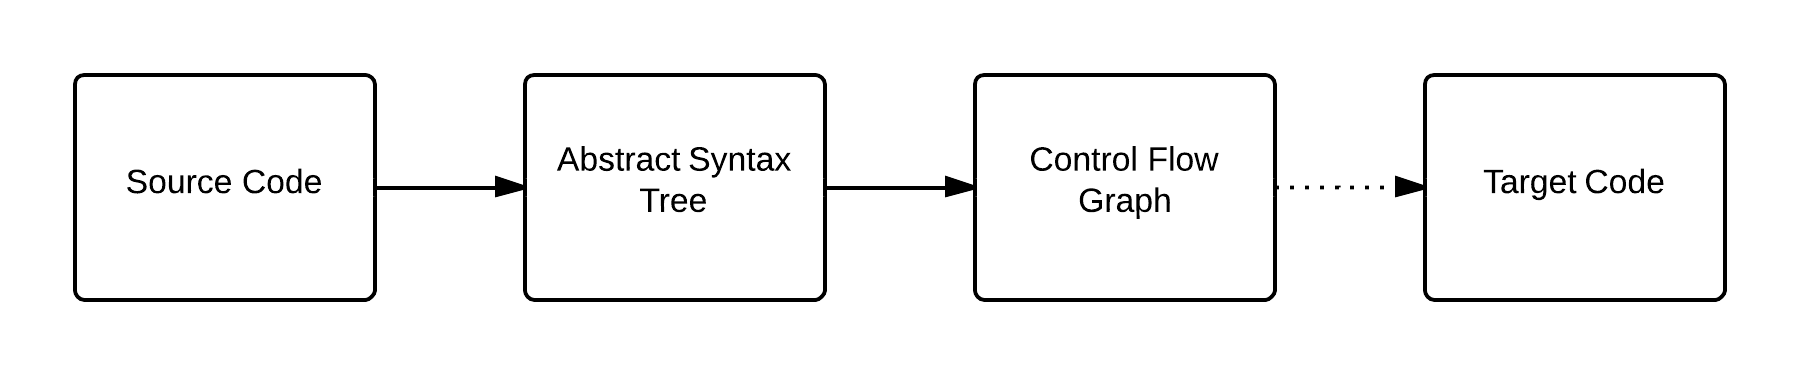
\includegraphics[width=0.8\linewidth]{figures/CompStructure}
\caption{Intermediate Representations}
\label{fig:Compiler}
\end{figure}

We divide the problem of translating the source program to target code into three stages. The first stage is to traverse the given AST and transform it to a more low-level intermediate representation which is Control Flow Graph (CFG); the steps are depicted in Figure 1.1. This thesis covers the design of the algorithm and implementation to transform the AST into CFG. A sample Scala program with control flow and iteration is presented in this chapter to show the process and result. The second stage is to analyze the CFG and identify the data dependencies between each block of the graph. In the end, we generate the executable code for the underlying system. The driver program of the WMS will then execute this code. The design of the algorithm and expected result of the last two stages are also delivered in this thesis. 

\section{Scala AST}
This section gives necessary introduction to AST to allow the reader to understand the transformation process from the source language to the target language. AST is one of the most important intermediate representations. During parsing, compiler creates syntax-tree nodes to represent significant programming constructs. As analysis continues, information is added to the node in the form of attributes associated to the node depending on the translation to be performed \cite{lam2006compilers}. In this thesis, we do not create our own AST representation but reuse the Scala compiler's parser and type checker. Additionally, the Scala compiler also provides a tool to traverse and transform an AST \cite{stocker2010scala}. 

Scala AST or Trees are the basis of abstract syntax which is used to represent programs. The Scala compiler uses AST as an intermediate representation before generating bytecode \cite{demarne2014scala}. In Scala reflection, Trees can be produced or used by the following APIs \cite{symboltreestypes}.

\begin{itemize}
\item Scala annotations. This API uses AST to represent their arguments and is exposed in \texttt{Annotation.scalaArgs}. 
\item \texttt{reify}. This special method takes an expression and returns an AST that represent this expression.
\item Compile time reflection with macros \cite{scalamacros} and runtime compilation with toolboxes use trees as their program representation medium. Macros expand trees at compile time allowing programmers to hack and manipulate AST within the compilation scope \cite{burmako2013scala}. 
\end{itemize} 

\subsection{AST Classes}
This section introduces some of the concrete trees classes that are used in traversing the trees in our implementation. All concrete classes are case classes, thus their parameters are listed following the class name as follows \cite{stocker2010scala}. 
\begin{itemize}
\item \texttt{Block(stats: List[Tree], expr: Tree)}. A Block consists of a list of statements and returns the value of expr.
\item \texttt{ValDef(mods: Modifiers, name: Name, tpt: Tree, rhs: Tree)}. Val- ue definitions are all definitions of vals, vars (identified by the MUTABLE flag) and parameters (identified by the param flag).
\item \texttt{LabelDef(name: Name, params: List[Ident], rhs: Tree)}. The Label- Def tree is used to represent iteration, both $While$ and $Do-While$ iteration. The Scala language specification \cite{odersky2004scala} defines that the while loop expression \texttt{while(e1) e2} is typed and evaluated as if it is an application of \texttt{whileLoop(e1)(e2)} where the hypothetical function \texttt{whileLoop} is defined in Listing 1.1 below. 
\begin{lstlisting}[language=scala,caption=WhileLoop Function, label = whileloop]
def whileLoop(cond: => Boolean)(body: => Unit): Unit = if (cond) { body ; whileLoop(cond)(body) } else {}
\end{lstlisting}
\item \texttt{Assign(lhs: Tree, rhs: Tree)}. Assign trees are used for non-initial assignments to variables. The lhs typically consists of an Ident(name) and is assigned the value of the rhs which normally contains an application (Apply) of a function. 
\item \texttt{If(cond: Tree, thenp: Tree, elsep: Tree)}. An If statement consists of three parts: the condition, the then part and the else part. If the else part is omitted, the literal () of type Unit is generated and the type of the conditional is set to an upper bound of Unit and the type of the then expression, usually Any.
\end{itemize}

\subsection{Generating Scala AST}
Scala macros is used in this thesis to lift the root Block of a Scala program into a monatic comprehension of intermediate representation. We present a sample Scala program with iteration and an If statement inside the iteration (refer to Listing 1.2) and show the generated Scala AST of the program. 
\\
\begin{lstlisting}[language=scala, caption=Workflow with Conditional, label = workflow2]
val e1 = DataSource("/tmp/input1.txt", CsvInputFormat[(String, Int, Int)]()).filter(x => x._1 == "Joshua")
val e2 = DataSource("/tmp/input2.txt", CsvInputFormat[(String, Int, Int)]()).filter(x => x._1 == "Marten")
var e3: DataSet[(String, Int, Int)] = null
var i = 0

while(i < 0) {
if (e1.map(x => x._2).reduce((x, y) => Math.max(x, y)).fetch().head > 50)
        e3 = e1.map { x => (x._1, x._2 + 1000, x._3)}
    else
    	e3 = e2.map { x => (x._1, x._2 + 1500, x._3)}
    }

val e4 = e3.write("/tmp/output.txt", CsvOutputFormat[(String, Int, Int)]())

e4
\end{lstlisting}

As shown in Scala AST in Figure 1.2, the program is represented by a Block which consists of list of statements and an expression which holds the final return value. Each of the variable definition is presented by a ValDef. The LabelDef in the AST represent the While statement in the program and consists of a name and a rhs of type If. The If statement consists of the three parts: condition, then part, and else part. In the while or LabelDef case, the else part which is of type Literal only contains an empty constant value. The then part is expanded to another list of statements and expression. Given that in the sample Scala program, there is a control flow inside the body of the loop, the statement then consists of another If statement. The then and else part of this If statement are of type Assign since in the program we assign a map function in the rhs to a variable name in the lhs. 

\begin{figure}[h!]
\centering
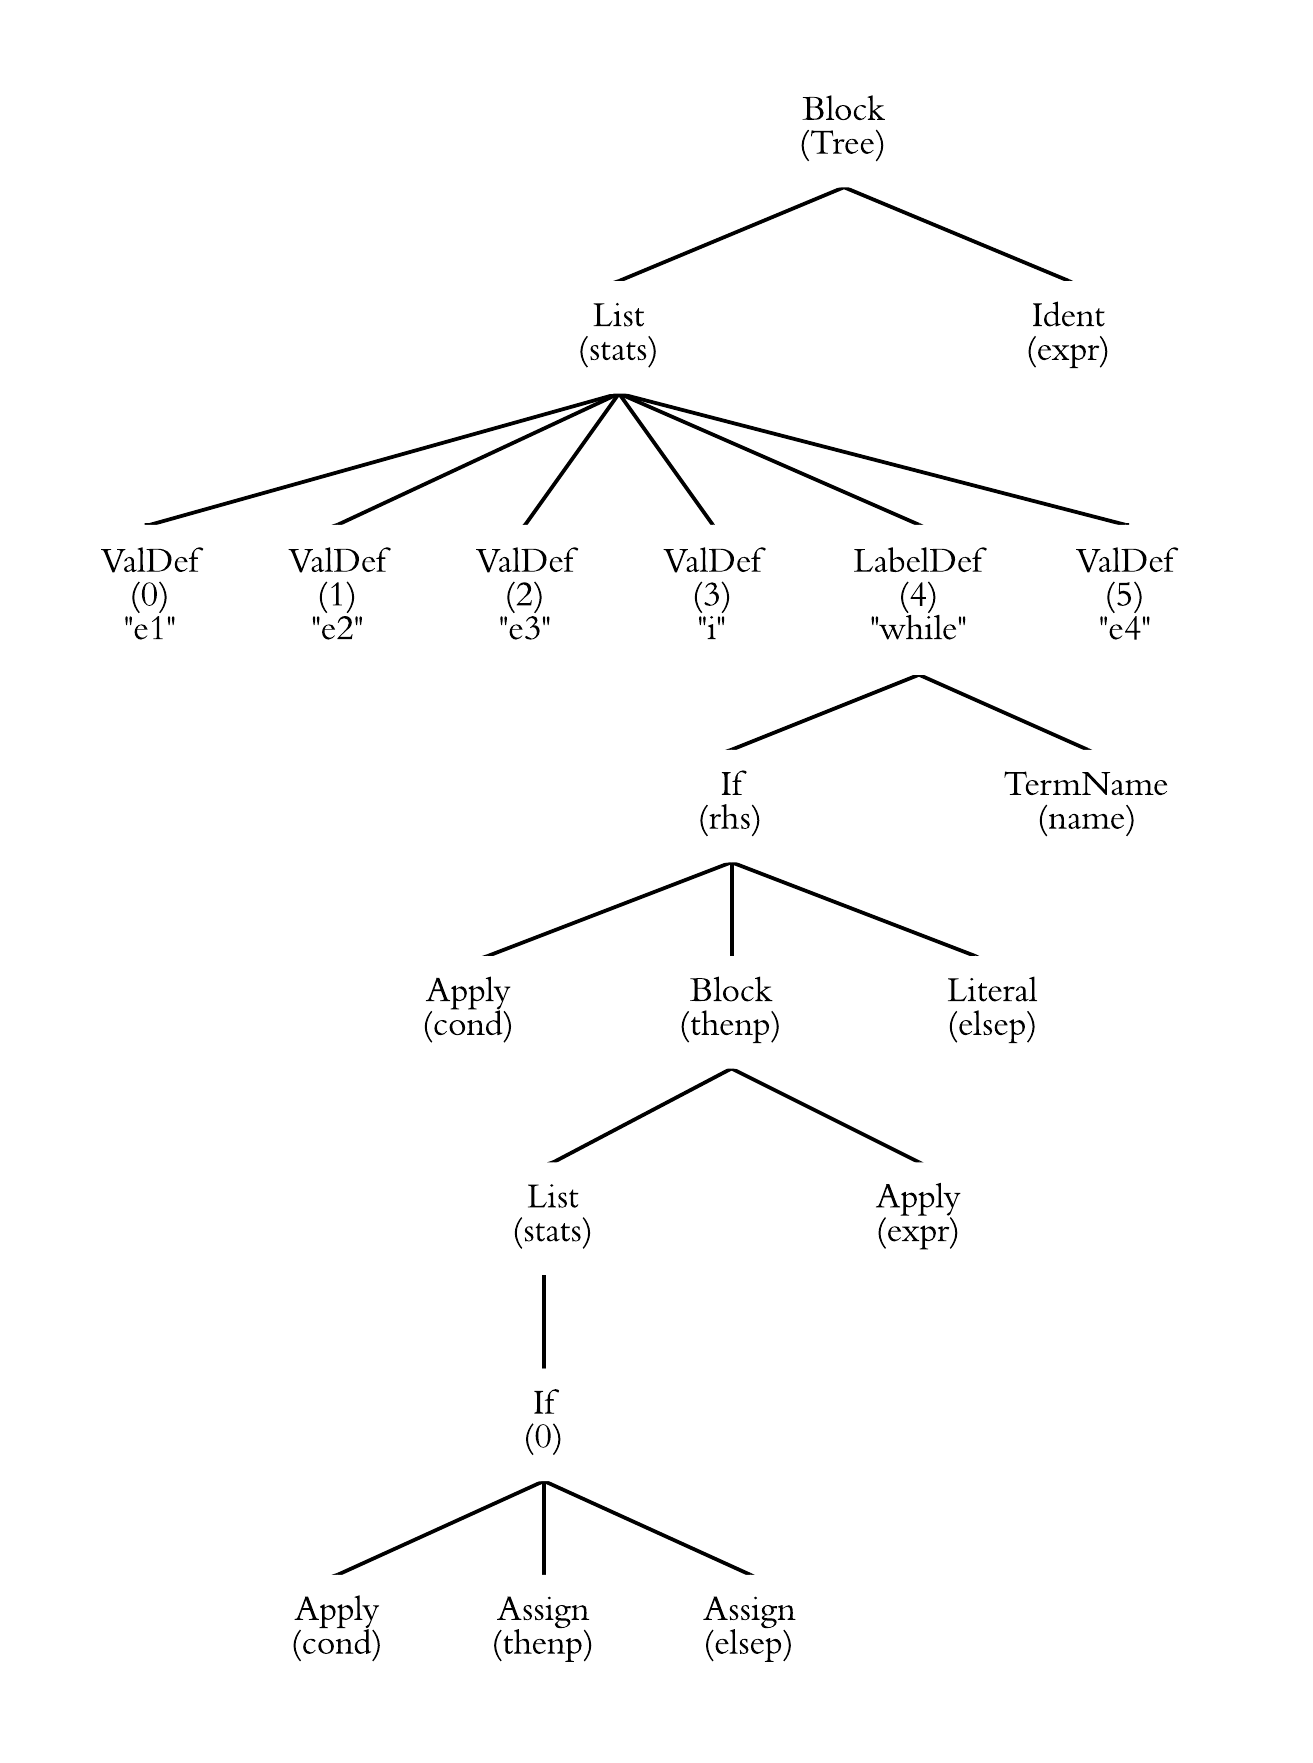
\includegraphics[width=0.8\linewidth]{figures/Tree}
\caption{Scala AST}
\label{fig:Tree}
\end{figure}

\section{CFG Definition}
The CFG is another intermediate representation that is produced from Scala AST in the first stage of the algorithm. Frances E. Allen \cite{allen1970control} defines a CFG as "a directed graph in which the nodes represent basic blocks and the edges represent control flow paths". CFG serves as framework for static analysis of program control flow. Many code generators partition intermediate representation instructions into basic blocks, which consist of sequences of instructions or statements that are always executed together \cite{lam2006compilers}. Basic blocks are a straight line, single-entry code with no branching except at the end of the sequence. 

\begin{figure}[h!]
\centering
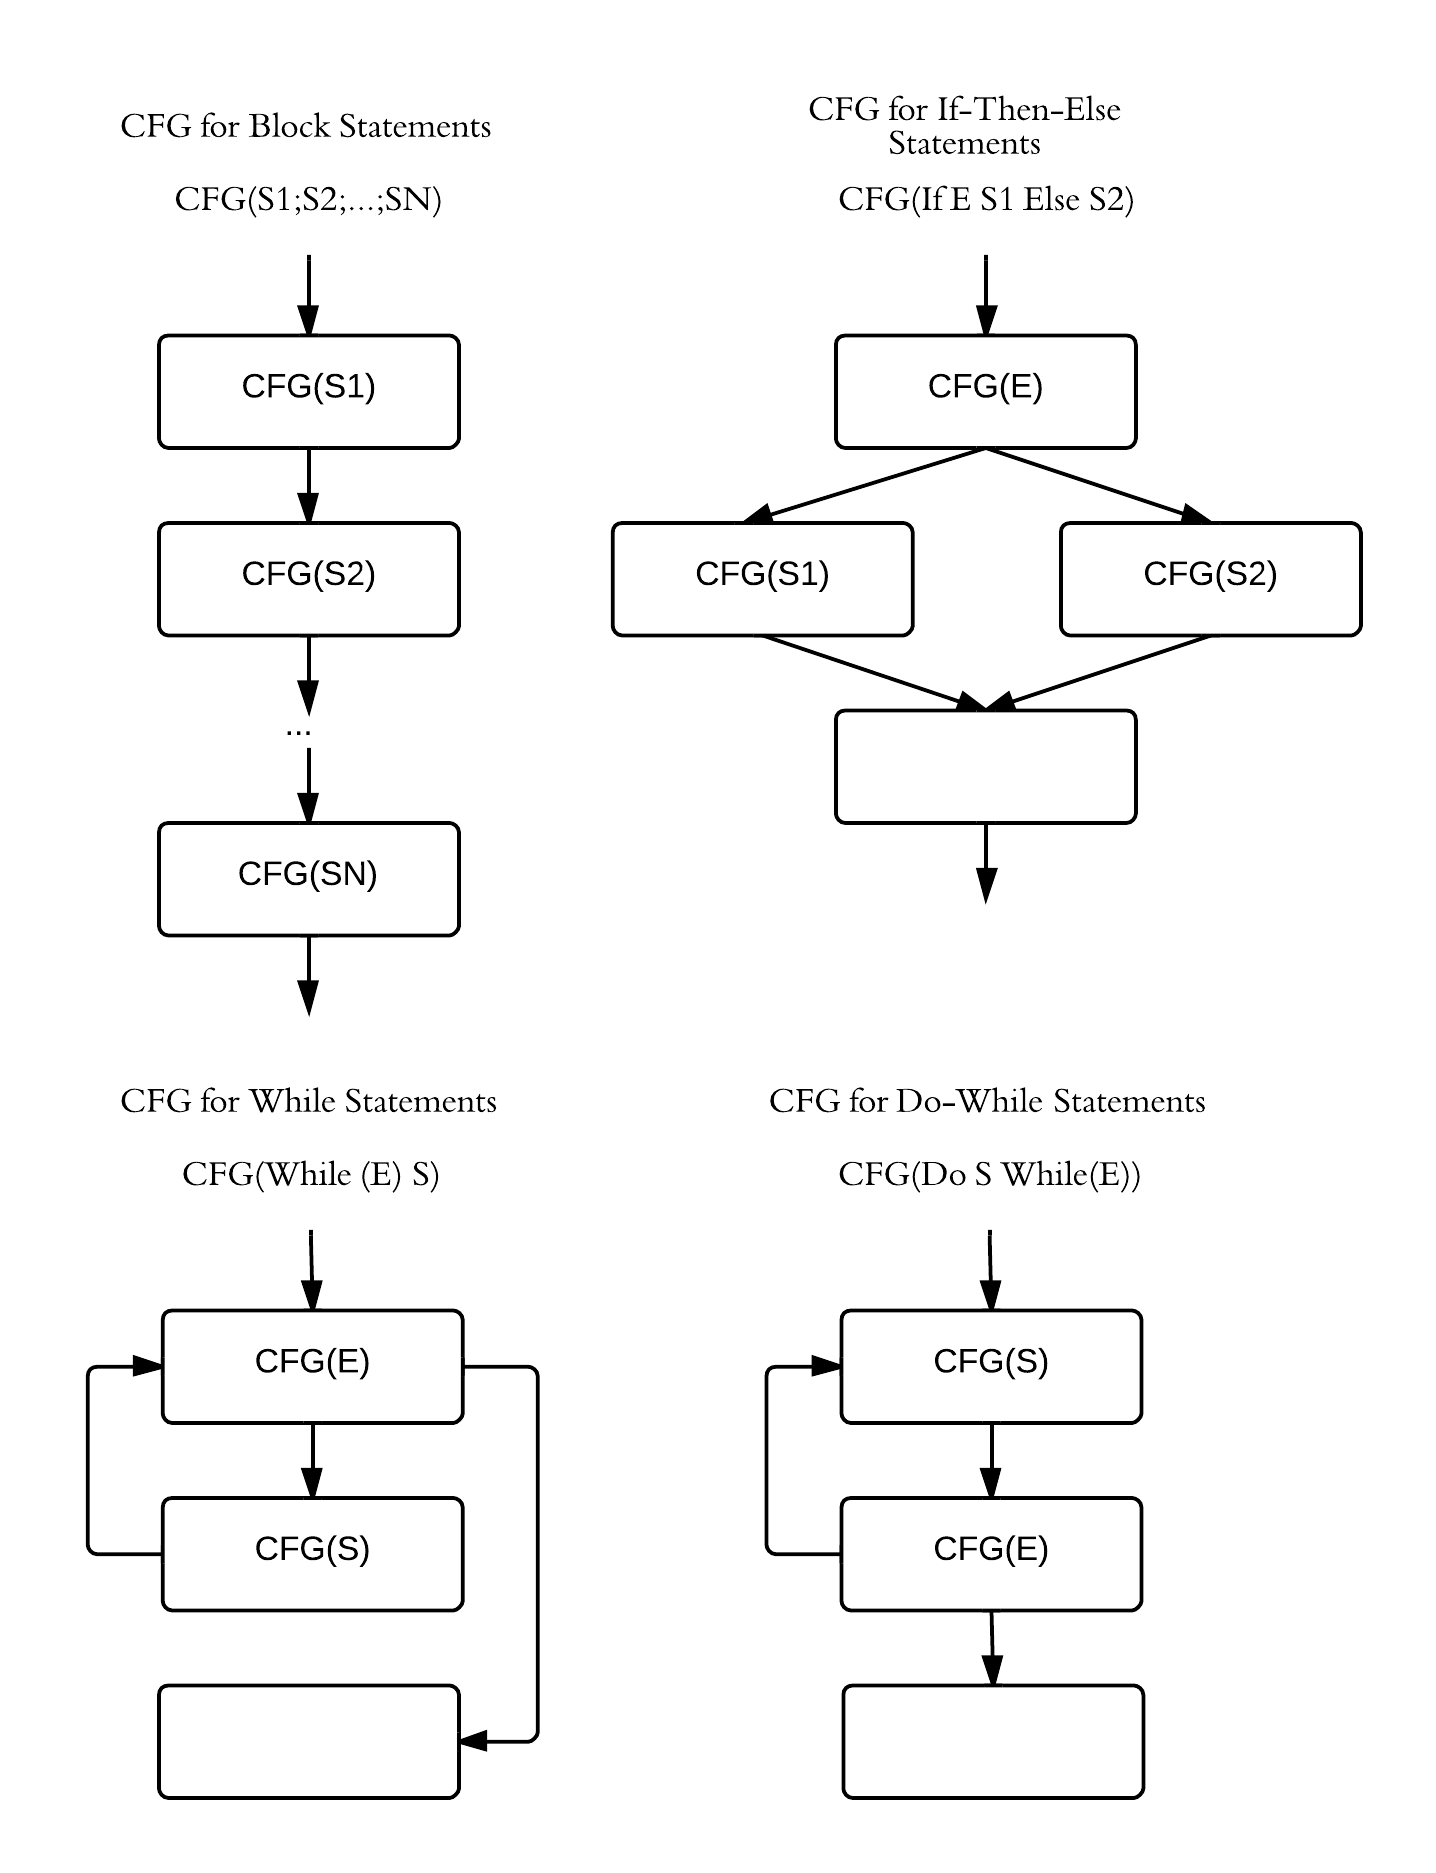
\includegraphics[width=0.7\linewidth]{figures/Graph}
\caption{CFG of Various Statements}
\label{fig:Graph}
\end{figure}

Edges represent possible flow of control from the end of one block to the beginning of the other. There may be multiple incoming or outgoing edges for each block \cite{allen1970control}. After the intermediate code has been partitioned into basic blocks, the flow of control between them can be represented by a CFG. There is an edge from block A to block B if and only if it is possible for the first statement in block B to immediately follow the last statement in block A. Given a Block statement, If-Then-Else statement, and While-statement, we formulate the expected CFG result from the first stage of the algorithm as shown in Figure 1.3. In the second stage of our algorithm, we analyze the graph to detect data dependencies and subsequently add another type of Edges which show the data dependencies between the nodes of the CFG. 

\section{Create CFG from AST Algorithm}
Creating CFG from AST is the first stage of the intermediate code and code generation process. This algorithm takes as an input a Scala AST and produces the output of a lower-level intermediate representation CFG $G=(V,E)$ with set $V$ of vertices and a set $E$ of directed edges. Each vertex $V$ is a sequence of one or multiple nodes $n$ in the AST. 

The idea is to traverse the tree from top to bottom starting from the $root$ and to visit each node $n$ of the children recursively. We check the type of each node $n$ and perform a set of actions accordingly. The procedure $createCFG(nCurr, G, vCurr, X)$ takes as input the following parameters. 
\begin{itemize}
\item $nCurr$ refers to the node that is currently being visited in the AST. In the beginning, $nCurr$ is initialized to root of the full AST of the program. Since we traverse the tree from top to bottom, the $nCurr$ becomes the root of the subtree of the initial root node. Depending on the type of the Tree, the $nCurr$ is either pushed to the current Vertex $vCurr$ or the subtree of the $nCurr$ is visited recursively. 

\item $G=(V,E)$ refers to the CFG produced by the procedure and is continuously being updated whenever recursion takes place. The CFG consists of a set of vertices and a set of directed edges. Each vertex of the resulted CFG is a sequence of statements or nodes in the AST. The vertices set $V$ of the graph has initial member of $vCurr$ whereas the edges set $E$ is initialized to an empty set.   

\item $vCurr$ refers to the vertex of the CFG that is currently being built. If the $nCurr$ or a subtree does not contain control flow or branches, the $nCurr$ will be pushed to the $vCurr$. Subsequently, if the subtree contains branches or control flow, new vertex will be added to the CFG as well as directed edges from the $vCurr$ to the new vertex. Furthermore, the new vertex will become the new $vCurr$ and the whole procedure of checking $nCurr$ for control flow is repeated. In the initialization, $vCurr$ is set to empty sequence since we just begin to traverse the tree. 

\item $X$ is a stack to store the variable which contains branches and needs to be updated with the return value of either the then part or the else part of the control flow. In the algorithm, this variable will be re-assigned to the return value and will be deleted from the stack allowing the stack empty at the end of the procedure.  

\end{itemize}

\begin{algorithm}[h]

\caption{Creating Control Flow Diagram from AST Part 1}\label{CFG}
\begin{algorithmic}[1]
\Initialize { $v_{curr}\gets [ ],V\gets \{v_{curr}\},E\gets \emptyset,X\gets [ ], n_{curr}\gets root$}
\Procedure{createCFG}{$n_{curr},G,v_{curr},X$}
\Switch {$n_{curr}$}
  \Case {$Block(stats,expr)$}
  	\For {each $s$ in $stats$}
  	\State $(G,v_{curr},X)\gets \Call{createCFG}{s,G, v_{curr},\emptyset}$
   	\EndFor  
    \State $(G,v_{curr},X)\gets \Call{createCFG}{expr,G, v_{curr},X}$
       	\State \textbf{return} $(G,v_{curr},X)$
      \EndCase
       
  \Case {$ValDef(name, rhs)$}
  		\If {$containsBranches(rhs)$}
  			\State $\Call{push}{ValDef(name,\emptyset),v_{curr}} $
  			\State $\Call{push}{name,X} $
  			\State $(G,v_{curr},X)\gets \Call{createCFG}{rhs,G, v_{curr},X} $
  		\Else
  			\State $\Call{push}{n_{curr}, v_{curr}} $
  		\EndIf
  	\State \textbf{return} $(G,v_{curr},X)$
  \EndCase

  \Case {$Assign(name,rhs)$}
    	\If {$containsBranches(rhs)$}
    		\State $\Call{push}{name,X} $
    		\State $(G,v_{curr},X)\gets \Call{createCFG}{rhs,G, v_{curr},X} $

    	\Else
    			\State $\Call{push}{n_{curr}, v_{curr}} $
    		\EndIf
    	\State \textbf{return} $(G,v_{curr},X)$
  \EndCase
  \Case {$While(cond,body)$}
  	\State $v_{condStart} \gets \Call{newV}$
  	\State $V \gets V \cup \{v_{condStart}\}; E \gets E \cup \{(v_{curr},v_{condStart})\}$ 
  	\State $(G,v_{condEnd},X)\gets \Call{createCFG}{cond,G,v_{condStart},\emptyset} $
  	\State $v_{bodyStart} \gets \Call{newV}{ }$
  	\State $V \gets V \cup \{v_{bodyStart}\}; E \gets E \cup \{(v_{condEnd},v_{bodyStart})\}$
  	\State $(G,v_{bodyEnd},X)\gets \Call{createCFG}{body,G, v_{bodyStart},\emptyset} $
  	\State $v_{curr} \gets \Call{newV}{ }$
  	\State $V \gets V \cup \{v_{curr}\}; E \gets E \cup \{(v_{condEnd},v_{curr}),(v_{bodyEnd},v_{condStart})\}$
  	\State \textbf{return} $(G,v_{curr},X)$
  \EndCase
 \algstore{bkbreak}
 \end{algorithmic}
 \end{algorithm}
 \begin{algorithm}
 \addtocounter{algorithm}{-1}
 \caption{Creating Control Flow Diagram from AST Part 2}\label{CFG2}
 \begin{algorithmic}[1]
 \algrestore{bkbreak}
  \Case {$DoWhile(cond,body)$}
      	\State $v_{bodyStart} \gets \Call{newV}{ }$
      	\State $V \gets V \cup \{v_{bodyStart}\}; E \gets E \cup \{(v_{curr},v_{bodyStart})\}$
  	\State $(G,v_{bodyEnd},X)\gets \Call{createCFG}{body,G, v_{body},\emptyset} $
  	\State $v_{condStart} \gets \Call{newV}{ }$
      	\State $V \gets V \cup \{v_{bodyEnd}, v_{condStart}\}; E \gets E \cup \{(v_{bodyEnd},v_{condStart})\}$ 
      	\State $(G,v_{condEnd},X)\gets \Call{createCFG}{cond,G,v_{cond},\emptyset} $
      	\State $v_{curr} \gets \Call{newV}{ }$
      	\State $V \gets V \cup \{v_{curr},v_{condEnd}\}$
      	\State $E \gets E \cup \{(v_{condEnd},v_{curr}),(v_{condEnd},v_{bodyStart})\}$
      	\State \textbf{return} $(G,v_{curr},X)$
    \EndCase
  \Case {$If(cond,thenp,elsep)$}
  	\State $(G,v_{cond},X)\gets \Call{createCFG}{cond,G, v_{cond},\emptyset}$
  	\State $v_{thenp} \gets \Call{newV}{ }$
  	\State $V \gets V \cup \{ v_{thenp}; E \gets E \cup \{(v_{curr},v_{thenp})\}$
  	\State $(G,v_{thenp},X)\gets \Call{createCFG}{thenp,G, v_{thenp},X} $
  	
  	\State $v_{elsep} \gets \Call{newV}{ }$
  	\State $V \gets V \cup \{v_{elsep}\};E \gets E \cup \{(v_{curr},v_{elsep})$
  	\State $(G,v_{elsep},X)\gets \Call{createCFG}{elsep,G, v_{elsep},X} $
  	
  	\State $v_{curr} \gets \Call{newV}{ }$
  	\State $V \gets V \cup \{v_{curr}\};E \gets E \cup \{(v_{thenp},v_{curr}),(v_{elsep},v_{curr})\}$
 	  	
  	\State \textbf{return} $(G,v_{curr},X)$
    	
  \EndCase

  \Case { $\_$}
  	\If {$X \neq \emptyset$}
	\State $name \gets X.head$
  	\State $\Call{push}{Assign(name,n_{curr}),v_{curr}} $ 
  	\Else
  	\State $\Call{push}{n_{curr},v_{curr}} $ 
  	\EndIf 
  	\State \textbf{return} $(G,v_{curr},X)$
  	
  \EndCase
 
\EndSwitch
\EndProcedure
\Procedure{containsBranches}{$n_{curr}$}
\Switch {$n_{curr}$}
  \Case {$Block(_,expr)$}
  \State $\Call{containsBranches}{expr}$
  \EndCase
  \Case {$If(\_)$}
  	\State \textbf{return} $true$
  \EndCase
  \Case {$\_$}
    \State \textbf{return} $false$
    \EndCase
\EndSwitch
\EndProcedure
\end{algorithmic}
\end{algorithm}

Using Scala pattern matching, we are able to traverse the tree and match the current node of the tree $nCurr$ to a Scala AST type. Based on its type, the following procedure will be taken. 

\begin{itemize}

\item $Block(stats, expr)$.
A Block typically consists of a list of statements and an expression. For every statement inside the Block, the procedure is called recursively and the Graph $G=(V,E)$, current vertex $vCurr$, and stack of variable $X$ are subsequently updated. After each statement is visited, the procedure is also called recursively for the single expression.  

\item $ValDef(name,rhs)$
As mentioned in the Scala AST introduction section, ValDef refers to definition of a variable both immutable (val) and mutable (var). In this case, we check whether the ValDef contains branches or control flow. If there is a control flow inside the ValDef, the same ValDef with a mutable identifier is pushed to the current vertex $vCurr$ and the name of the variable of type TermName is stored in the stack variable $X$. The name of the variable needs to be stored because it must be assigned later on with the value in the Then part or the Else part of the control flow. The rhs then becomes the current node $nCurr$ and the procedure is called recursively.  Sample program that will encounter this case is provided in the Listing 1.3 below. In this case, the variable $e3$ is stored in $X$ and later will be assigned to the function "e1.map {..}" or function "e2.map {..}".
\begin{lstlisting}[language=scala,caption=ValDef with Branches, label = valdef]
val e3 = if (e1.map(x => x._2).reduce((x, y) => Math.max(x, y)).fetch().head > 50)
	e1.map { x => (x._1, x._2 + 1000, x._3)}
else
	e2.map { x => (x._1, x._2 + 1500, x._3)}
\end{lstlisting}

If the ValDef does not contain branches, then the current node $nCurr$ is simply pushed to the current vertex $vCurr$. 

\item $Assign(name,rhs)$
The procedure for the case Assign is similar with ValDef. We check whether the tree or node contains branches. If it does, the name of the variable is stored in the stack variable $X$ to be assigned later on with the value in the Then part or the Else part of the control flow. The procedure is then called recursively with the rhs as the new current node $nCurr$. Similar to ValDef, if the Tree does not contain branches, the current node $nCurr$ is simply pushed to the current vertex $vCurr$.

\item $While(cond,body)$
As depicted in Figure 2-3, for While loop, a new vertex $vCondStart$ is created to store the condition of the iteration. A directed edge is defined from the current vertex $vCurr$ to the new vertex $vCondStart$. A new vertex $vBodyStart$ is also created to store the statements in the $body$ of the iteration. Both the $cond$ and $body$ may or may not contain branches. Hence, recursive call both for $cond$ and $body$ take place which results in the new vertex $vCondEnd$ and $vBodyEnd$ respectively. A directed edge is defined from the end of the $body$ which is the vertex $vBodyEnd$ to the beginning of the $cond$ which is the vertex $vCondStart$. At the end, a new vertex is created as the new current vertex $vCurr$ and a directed edge is defined from the vertex $vBodyEnd$ to the new current vertex $vCurr$. 

\item $DoWhile(cond,body)$
The procedure for DoWhile case is similar with While case with the differences in the order the vertices are created as well as the directed edges connecting the vertices. The $vBodyStart$ is created first and is connected to the $vCurr$. The vertex result of the recursive call to the body of the iteration, vertex $vBodyEnd$ is connected to the new vertex $vCondStart$ which stores the condition of the iteration. The end of the condition $vCondEnd$ is connected to the start of the $body$ $vBodyStart$. Similar to the While loop, at the end, a new vertex is created as the new current vertex $vCurr$ and a directed edge is defined from the vertex $vCondEnd$ to the new current vertex $vCurr$. 

\item $If(cond,thenp,elsep)$
At first, we create a new vertex $vCond$ to store the condition of the If statement. A directed edge is connected from the current vertex $vCurr$ to the $vCond$. A recursive call is performed to the procedure since the $cond$ may or may not contain branches. We then create two new vertices $vThenp$ and $vElsep$ to represent the Then part and the Else part of the If statement consecutively. A directed edge is defined from $vCond$ to both new vertices $vThenp$ and $vElsep$ to represent all possible flows. Recursive call is performed both for the Then part $thenp$ and Else part $elsep$ since they may or may not contain branches. At the end, a new vertex is created as the new current vertex $vCurr$ and a directed edge is defined both from the vertex $vThenp$ and vertex $vElsep$ to the new current vertex $vCurr$. 

\item $Default Case)$
We first check whether the stack of variable $X$ contains any member. If yes, then we have get the last member inserted to $X$ which is a name, and assign the current node $nCurr$ to the name. This assignment is then pushed to the current vertex $vCurr$. If the stack variable $X$ does not contain any member, which means no assignment is needed, the current node $nCurr$ is simply pushed to the current vertex $vCurr$. 
\end{itemize}

We perform this algorithm with the input of the Scala AST of the program in Listing 2-1. The CFG result is shown in Figure 1.4. 

\begin{figure}[h!]
\centering
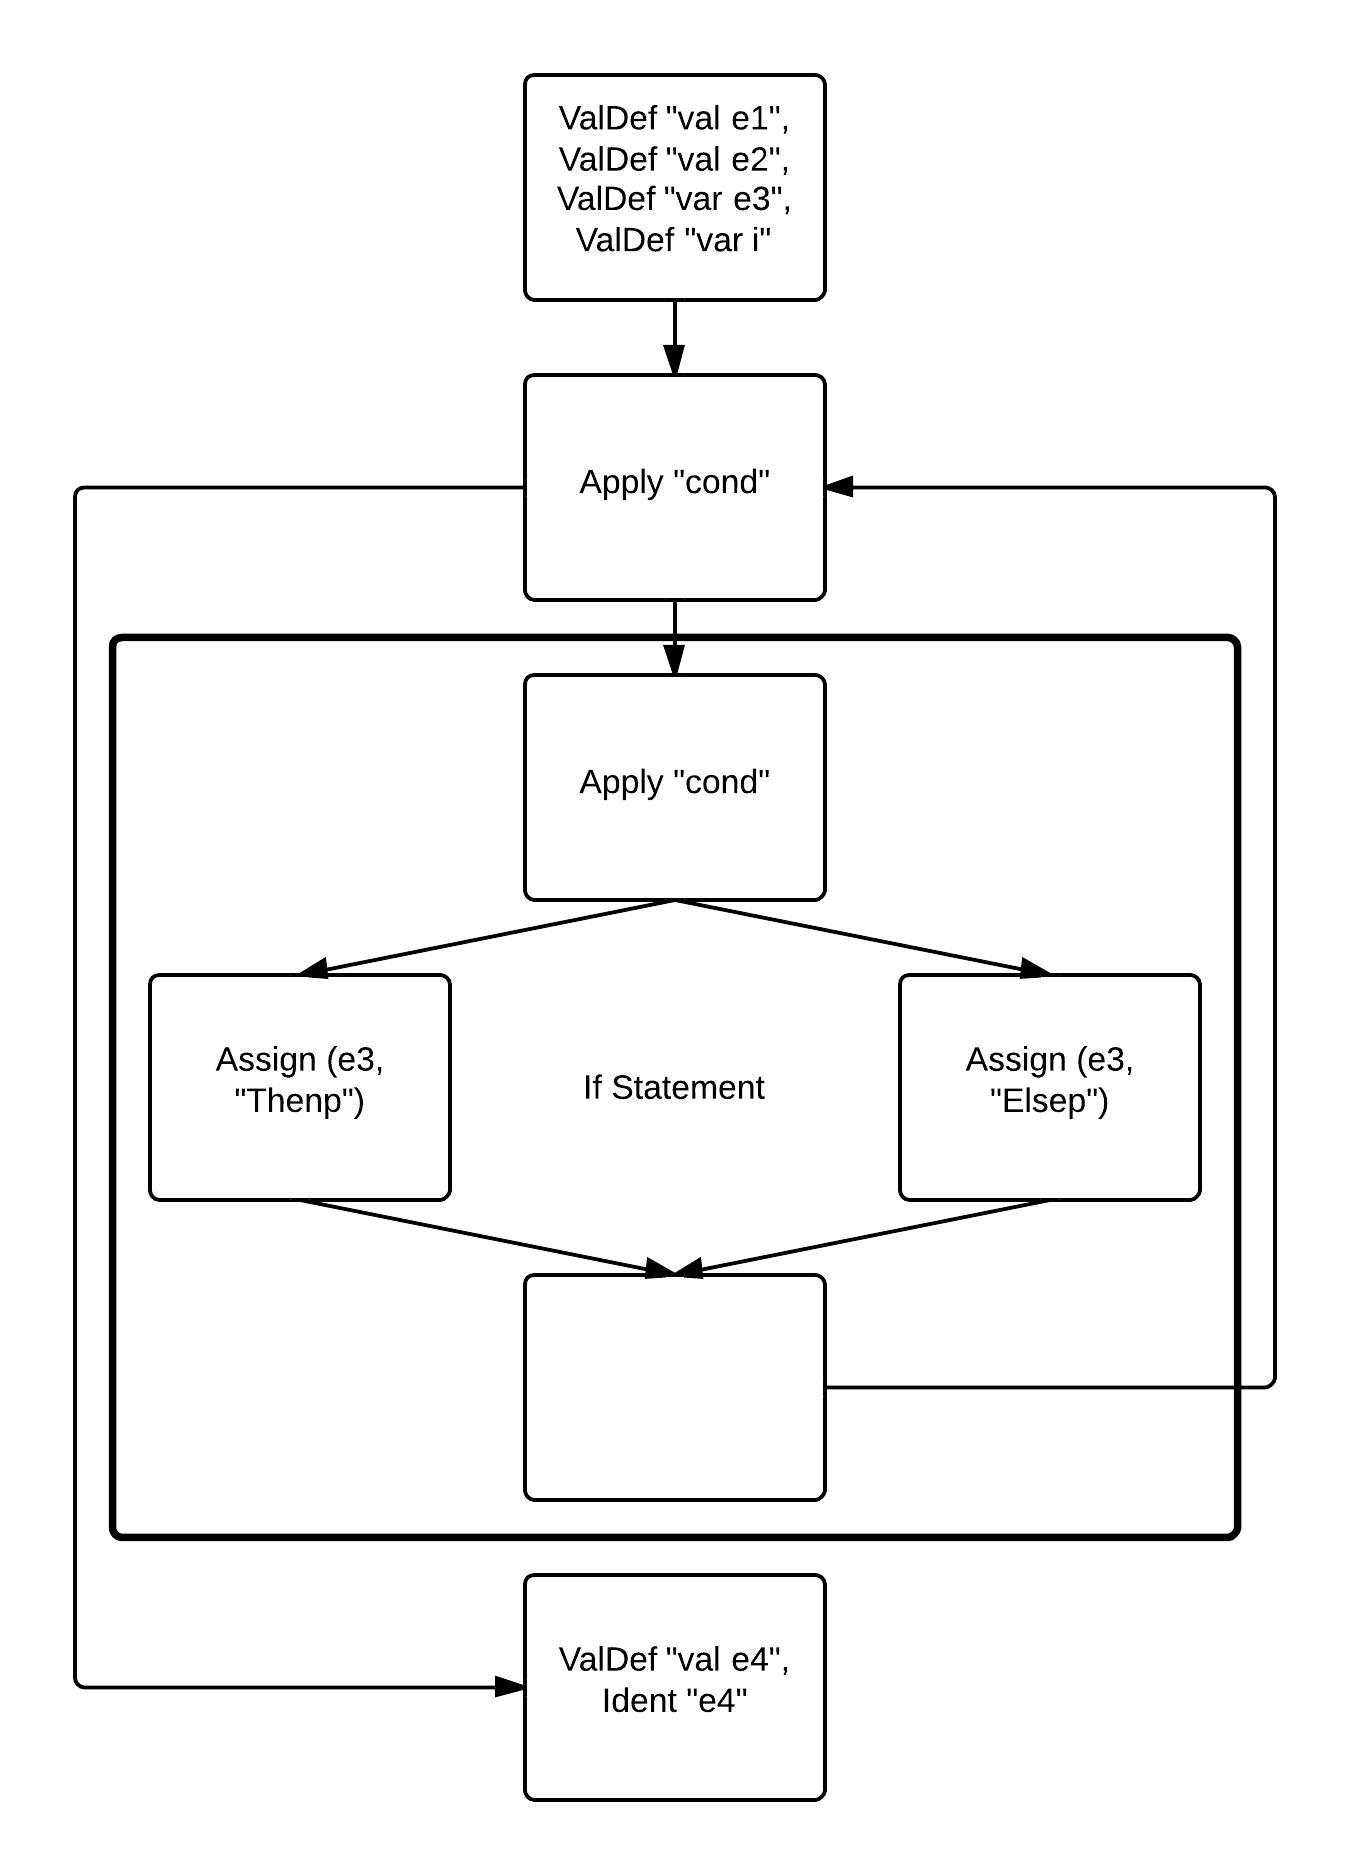
\includegraphics[width=0.7\linewidth]{figures/FinalGraph}
\caption{CFG of Scala AST of sample Program}
\label{fig:FinalGraph}
\end{figure}




\include{chap3}
\appendix
\include{app1}
%% This defines the bibliography file (main.bib) and the bibliography style.
%% If you want to create a bibliography file by hand, change the contents of
%% this file to a `thebibliography' environment.  For more information 
%% see section 4.3 of the LaTeX manual.
\begin{singlespace}
\bibliography{main}
\bibliographystyle{plain}
\end{singlespace}

\end{document}
